\newpage
\section{Graphene}
\subsection{Very brief history of graphene}
Graphene is the most well-known 2D-material in the world.  Explosion of great interest to this material happened after Andre Geim and Konstantin Novoselov in 2010 received Nobel Prize in Physics "for groundbreaking experiments regarding the two-dimensional material graphene" \cite{geim}. 

But story of graphene started long years ago. Already in 1859 D.C. Brodie discovers the highly lamellar structure of thermally reduced graphite oxide \cite{brodie}. At the beginning of XXth century crystal structure of graphite was solved with diffraction method \cite{debije, bernal} and properties of graphite oxide paper was studied \cite{haenni}.

The theory of graphene was first studied by P. R. Wallace in 1947 as a first step to describing electronic properties of 3D graphite \cite{wallace}. The massless Dirac equation was first formulated for graphene by David P. DiVincenzo and Eugene J. Mele in 1984 \cite{divincenzo}. Semenoff emphasized the occurrence in a magnetic field of an electronic Landau level precisely at the Dirac point. This level is responsible for the anomalous integer quantum Hall effect.

At the ed of XXth century single layers of carbon atoms where epitaxially grown on other bulk materials\cite{epitaxial}. However strong interaction between graphene grown in such way and substrate significantly affects electronic structure and properties of graphene. In 2004 Andre Geim and Konstantin Novoselov published their work on the scotch tape method witch allowed to produce single layers of graphene weakly bounded to substrate on relatively large scale\cite{geim-science}. This paper initiated a global explosion in graphene research.

\subsection{Geometry of graphene}
Graphene is one-atom-sick sheet of carbon atoms arranged in hexagonal as shown on fig. \ref{fig:graphene_lattice}. The lattice vectors can be chosen as 
\begin{equation}
	\vec{a_1} = \frac{a}{2} (3, \sqrt{3}), \qquad \vec{a_2} = \frac{a}{2} (3, - \sqrt{3}),
\end{equation}
where $a \approx 1.42 \AA$ is $C-C$ bond length. There are two carbon atoms per unit cell, let's name them $A$ and $B$.The three nearest-neighbor vectors in real space are given by 
\begin{equation}
	\vec{\delta_1} = a (1, 0), \quad \vec{\delta_2} = \frac{a}{2} (-1, \sqrt{3}), \quad \vec{\delta_3} = \frac{a}{2} (-1, -\sqrt{3})
\end{equation}
and point from atom of one kind to another, e.g. from $A$ to $B$ and vice versa.
The reciprocal space lattice are given by
\begin{equation}
	\vec{b_1} = \frac{2 \pi}{3 a}(1, \sqrt{3}), \qquad \vec{b_2} = \frac{2 \pi}{3 a} (1, -\sqrt{3})
\end{equation}
Of particular interest for physics of graphene are two points in reciprocal space at the corners of Brillouin zone (BZ):
\begin{equation}
	K = (\frac{2 \pi}{3 a}, \frac{2 \pi}{3 \sqrt{3}}), \qquad K' = (\frac{2 \pi}{3 a}, -\frac{2 \pi}{3 \sqrt{3}})
\end{equation}

\begin{figure}[ht] \label{fig:graphene_lattice}
\begin{center}
  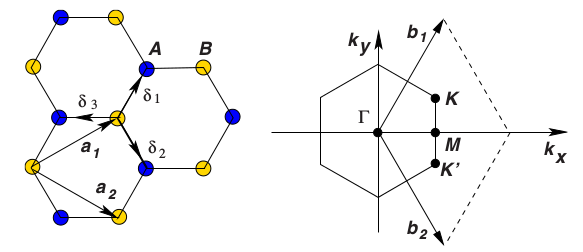
\includegraphics[width=0.55\linewidth]{img/graphene_lattice}
  \caption{Left: lattice structure of graphene. Right: corresponding Brillouin zone.}
\end{center}
\end{figure}

\subsection{Calculation of $\pi$ bands}
The easiest model one can use to describe electronic properties of graphene is TB model considering only $p_z$ orbitals for each carbon atom. All this orbitals are perpendicular to graphene plane and parallel to each other. They form $\pi$ bands. Band structure of graphene around the Fermi level is determined by the $\pi$ bands. 

Here I will take into account only interaction between nearest neighbors. One can also assume, that orbitals at different atoms are orthogonal to each other.

So to determine graphene band structure one should solve eigenvalue problem, where Hamiltonian matrix dimension is $2 \times 2$. The energy bands derived from this Hamiltonian have the form \cite{wallace}
\begin{equation}
	E(\vec{k}) = \pm V_{pp\pi}\sqrt{3 + 2 \cos\left(\sqrt{3} k_y a\right) + 4 \cos\left(\frac{\sqrt{3}}{2} k_y a\right) \cos\left(\frac{3}{2} k_x a\right)} 
\end{equation}

\begin{figure}[h] 
\begin{center}
  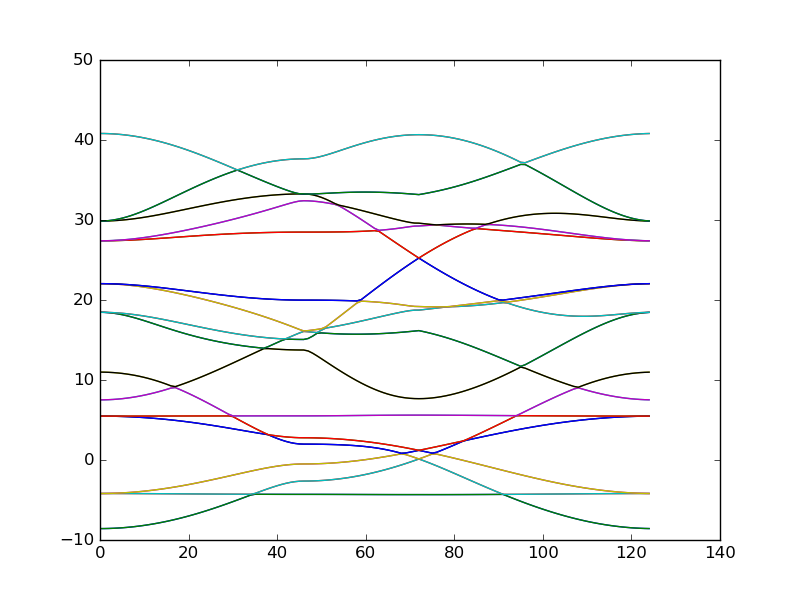
\includegraphics[width=0.55\linewidth]{img/graphene_pd_soc}
  \caption{Calculated Band structure of graphene ($p_3d_5$)).}
\end{center}
\end{figure}
\begin{figure}[h] 
\begin{center}
  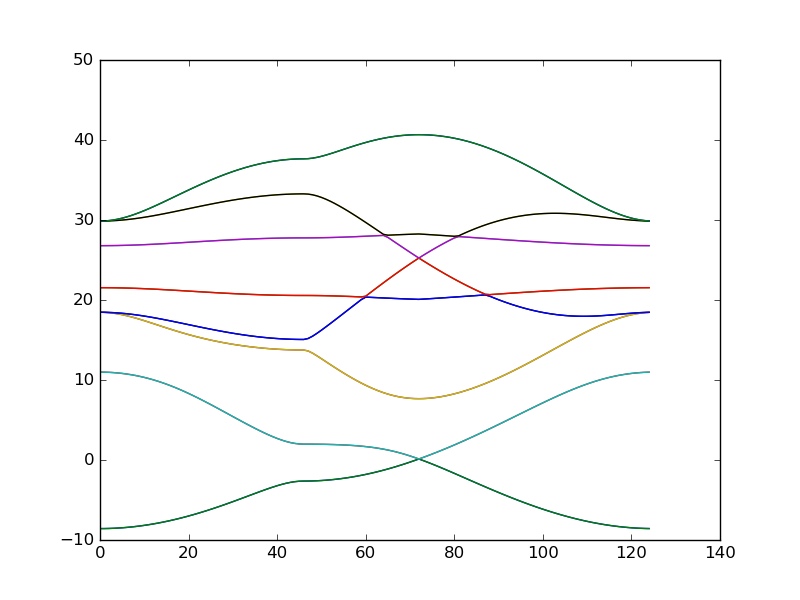
\includegraphics[width=0.55\linewidth]{img/graphene_pd_soc3}
  \caption{Calculated Band structure of graphene ($p_zd_{xz}d_{yz}$)).}
\end{center}
\end{figure}
